\ifx\headerIncludedJR\undefined
  \documentclass[11pt,a4paper]{article}
  \setlength{\textwidth}{5.50in}
  \usepackage[utf8]{inputenc}
\usepackage[T1]{fontenc}
\usepackage{amsmath}
\usepackage{amsthm}
\usepackage{amssymb}
%\usepackage{rotating}
%\usepackage{amslatex}
\usepackage{siunitx}
\usepackage{multicol}%for multicol
\usepackage{blkarray}%blockarray and block
\usepackage{comment}
\usepackage{fnbreak}%get a warning if a footnote is split
\usepackage[section]{placeins}
\usepackage{listings}
\lstset{breaklines=true,basicstyle=\ttfamily,language=Python}
\usepackage{arrayjobx}
\usepackage{array}%for \newcolumntype
%\usepackage[shortlabels]{enumitem}
\usepackage{mathtools}
\usepackage{afterpage}
\usepackage{setspace}% for \setstretch
\usepackage{algorithm}
\usepackage{algpseudocode}%for algorithmic
\usepackage{thmtools}%so that autoref works with Lemmas
\usepackage{tikz}
\usepackage{pgfplots}
\pgfplotsset{compat=1.15}
\usepackage{shuffle}
\usepackage{textcomp}%for \textrecipe
\usepackage{fontawesome}%for \faTable
\usetikzlibrary{calc,shapes,arrows.meta,decorations.markings,arrows}
\usetikzlibrary{graphs,positioning,svg.path,backgrounds}
\newcommand{\tikzmark}[1]{\tikz[overlay,remember picture] \node (#1) {};}
%\usepackage{CJKutf8}%for CJKChar

%\usepackage[backend=biber,backref=true]{biblatex}
\usepackage[backend=biber,style=alphabetic,backref=true,maxbibnames=10]{biblatex}
\addbibresource{sigs.bib}
\usepackage{url}

\usepackage{imakeidx}
%not a list of definitions, just symbols and abbreviations
%What is an abbreviation? Is QR? 
\makeindex[intoc,title=Symbols and abbreviations index]
\def\jind#1{\index{#1}}
\def\jindmath#1#2{\index{#2@$#1$}}
\def\jindv#1{\index{#1v@\texttt{#1}}}
%Some places I've given up and used \index in the text 
\definecolor{bluee}{rgb}{0.4, 0.4, 1.0}
%https://tex.stackexchange.com/questions/134191/line-breaks-of-long-urls-in-biblatex-bibliography
\setcounter{biburlucpenalty}{8000}
\setcounter{biburllcpenalty}{8000}

\usepackage{hyperref}

%so that autoref works with algorithms
\newcommand{\algorithmautorefname}{Algorithm}

%might help url breaking in bibliography
%\Urlmuskip=0mu plus 1mu minus 1mu
%also all the emergencystretch/looseness/fussy/sloppy
%to play with
%https://tex.stackexchange.com/questions/18505/how-to-use-sloppy-for-just-some-references

\def\ii{{\texttt{iisignature}}}
\def\pypi{{\texttt{PyPI}}}
\def\numpy{{\texttt{numpy}}}
\def\scipy{{\texttt{scipy}}}
\def\i#1{\index{#1@\texttt{#1}}}
\def \hilite#1{\underline{\color{blue}\textbf{#1}}}
%\def \alph#1{{\color{blue}\mathbf{#1}}}
\def \lex{<_L}
\def\kron{\underline{\otimes}}

\graphicspath{{C:/Users/Jeremy/Dropbox/phd/graphs/}{/home/jeremyr/Dropbox/phd/graphs/}{/Users/reizenstein/DropboxPersonalSymlink/phd/graphs/}}

%\RequirePackage{relsize}
%\DeclareRobustCommand\CXX{C\kern-.05em \raisebox{.3ex}{\scalebox{0.9}{\textbf{+\kern-.10em+}}}}
\DeclareRobustCommand\CXX{C\kern-.05em {\scalebox{0.9}{\textbf{+\kern-.10em+}}}}
%\DeclareRobustCommand\{\texorpdfstring{\CXX}{C++}}
\DeclareRobustCommand\CC{C\texttt{++}}
\def\bftab{\fontseries{b}\selectfont}
\newtheorem{theorem}{Theorem}
%\newtheorem*{theorem*}{Theorem}%bad idea, because you can't refer to it.
\newtheorem{definition}[theorem]{Definition}
%\newtheorem{outsideTheorem}[theorem]{Theorem}
\newtheorem{example}[theorem]{Example}
\newtheorem{conjecture}[theorem]{Conjecture}
\newtheorem{lemma}[theorem]{Lemma}
\newtheorem{proposition}[theorem]{Proposition}
\newtheorem{remark}[theorem]{Remark}

\newcommand{\area}{\mathsf{area}}
\newcommand{\Area}{\mathsf{Area}}
\newcommand{\emptyword}{\epsilon}
\newcommand{\ds}{d} % dimension of the signal
\newcommand{\TC}{T((\R^\ds))} % concat
\newcommand{\TS}{T(\R^\ds)} % shuffle
\newcommand{\GL}{\operatorname{GL}}
\newcommand{\SO}{\operatorname{SO}}
%\newcommand{\id}{\operatorname{id}}
\newcommand{\id}{\mathsf{id}}

\newcommand{\evaluatedAt}[1]{\,\raisebox{-.5em}{$\vert_{#1}$}}

\def\hssymbol{\mathbin{\succ}}
\def\hs#1#2{#1\hssymbol#2} %half shuffle
%\def\hs#1#2{z(#1,#2)} %half shuffle
\def\areab#1{\underline{\area}(#1)}
\def\areabb{\underline{\area}}
\newcommand{\R}{\mathbb{R}}
\newcommand{\Q}{\mathbb{Q}}
\newcommand{\C}{\mathbb{C}}
\newcommand{\N}{\mathbb{N}}
\newcommand{\spann}{\operatorname{span}}
\newcommand{\sign}{\operatorname{sign}}

\DeclareMathOperator*{\argmax}{arg\,max}
\DeclareMathOperator*{\argmin}{arg\,min}
\DeclareMathOperator{\softmax}{softmax}

%indicate that this file has been had
\def\headerIncludedJR{}
\def\endDocumentJR{}

%general hints
%https://homepages.inf.ed.ac.uk/imurray2/compnotes/latex.html

  %this cannot be in header.tex as it messes up
  %the thesis copyright page
  \def \alph#1{{\color{bluee}\mathbf{#1}}}
  \begin{document}
  \tableofcontents
  \def\endDocumentJR{\printindex \printbibliography[heading=bibintoc]\end{document}}
\fi

\let\word\alph
In this chapter I discuss some new results about signature elements which are invariant under certain transformations of the ambient space. 
Invariants to transformations which are known to be irrelevant for the problem at hand are potentially useful in machine learning as explained in
%Section~\ref{sec:invariants}.
\autoref{sec:invariants}.


\section{Signatures versus FKK expressions}
\label{sec:fkk}
There is a vast literature on invariants of curves, mostly in two dimensions.
Among the techniques used, the method of ``integral invariants'' 
of \cite{FKK}\jind{FKK}, which has been used for example in \cite{useFKK} for character recognition, is close to our iterated-integral signature method. 
Their method has not been explicitly compared with our iterated-integral signature.
%
In that work, for a curve $X: [0,T] \to \R^\ds$, $\ds=2,3$,
the building blocks for invariants are expressions of the form
\begin{align}
  \label{eq:expression}
  \int_0^T (X^1_r)^{\alpha_1} \dots (X^\ds_r)^{\alpha_\ds} dX^i_r, \qquad i=1,..,\ds.
\end{align}
for nonnegative integers $\alpha_1\dots\alpha_d$.
This can be written using the shuffle identity \eqref{eq:shuffle} in terms of the signature $S(X)_{0,T}$ as follows.%
\footnote{I write $a^{\shuffle n}$ for $\overbrace{a\shuffle\dots\shuffle a}^{\text{$n$ times}}$, which is well-defined because the shuffle product is associative.\jindmath{\cdot^{\shuffle n}}{shan}}
\begin{align}
  \int_0^T &(X^1_r)^{\alpha_1} \dots (X^\ds_r)^{\alpha_\ds} dX^i_r\nonumber
  \\&=\int_0^T \langle S(X)_{0,r},\alph 1^{\shuffle\alpha_1}\rangle\dots\langle S(X)_{0,r},\alph {\ds}^{\shuffle\alpha_{\ds}}\rangle\,dX^i_r\nonumber
\\ &=\int_0^T \langle S(X)_{0,r},\alph 1^{\shuffle\alpha_1}\shuffle\dots\shuffle\alph {\ds}^{\shuffle\alpha_{\ds}}\rangle\,dX^i_r\nonumber
\\ &=\langle S(X)_{0,T},(\alph 1^{\shuffle\alpha_1}\shuffle\dots\shuffle\alph {\ds}^{\shuffle\alpha_{\ds}})i\rangle
\\ &=\alpha_1!\dots\alpha_\ds!\langle S(X)_{0,T},(\alph 1^{\alpha_1}\shuffle\dots\shuffle\alph {\ds}^{\alpha_{\ds}})i\rangle
\end{align}
These building blocks, then, are the signature elements which are a shuffle of letters concatenated with a single letter. These are exactly the signature elements which show up when defining an integral of a one form along a path.
%By the shuffle identity (Lemma~\ref{lem:shuffleIdentity}) these values can be found in the signature $S(X)_{0,T}$.
%
We note that the building blocks %expressions of the form \eqref{eq:expression}
are \emph{not} enough to uniquely characterize a path, unlike iterated-integral signatures.
Indeed, the following lemma gives a counterexample to the conjecture on p.906 in \cite{FKK}
that ``signatures of non-equivalent curves are different''
(here, the ``signature'' of a curve means the set of expressions of the form \eqref{eq:expression}). The idea for the counterexample is that the the whole of the first two levels of the signature, but not the third, is included in the form \eqref{eq:expression}, so a good choice would be something like a figure of eight, which has nothing on the first two levels, and it makes sense to pick a curve which has a tractable form.
\begin{lemma}
  Consider the two closed curves $X^+$ and $X^-$ in $\R^2$, given for $t$ in $[0,2\pi]$ as%
  %\footnote{
  %  The images of both these curves coincide
  %  and form an algebraic curve, called the ``lemniscate of Gerono''.}
  \begin{align*}
    X^{\pm,1}_t &=\pm\cos t\\
    X^{\pm,2}_t &=\sin 2t.
  \end{align*}

  Then all the expressions \eqref{eq:expression} coincide on $X^+$ and $X^-$.
  %even though they are \emph{not} equal as curves up to tree-likeness, translation and rotation.
\end{lemma}

These curves both trace a figure called the \emph{lemniscate of Gerono} which is illustrated in Figure~\ref{fig:lemniscate}, but in different ways.
\begin{figure}
\begin{center}
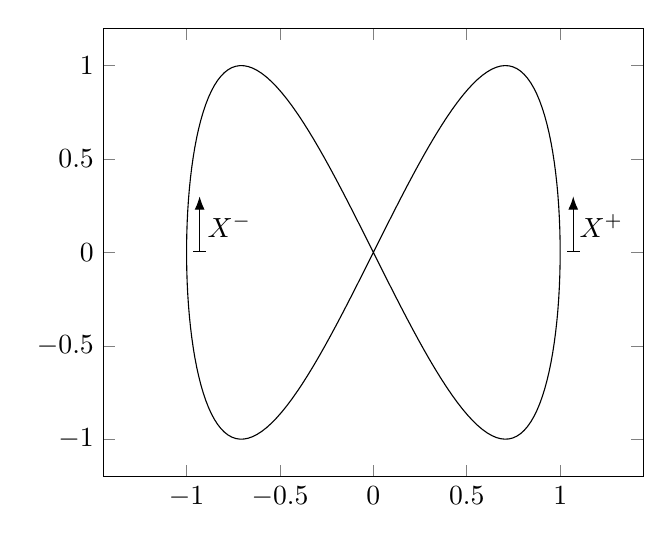
\begin{tikzpicture}
\begin{axis}[
trig format plots=rad,
axis equal,
%    hide axis
]
\addplot [domain=0:2*pi, samples=200, black] ({cos(x)}, {sin(2*x)});
\draw[|-Latex] (axis cs:1.07,0)--(axis cs:1.07,0.3);
\node at (axis cs: 1.22,0.14) {$\displaystyle X^+$};
\draw[|-Latex] (axis cs:-0.93,0)--(axis cs:-0.93,0.3);
\node at (axis cs: -0.77,0.14) {$\displaystyle X^-$};
\end{axis}
\end{tikzpicture}
\end{center}	
	\caption[The lemniscate of Gerono.]{\label{fig:lemniscate}The lemniscate of Gerono. Traversing it once
    from each of the two starting points
  indicated gives two distinct closed curves with distinct iterated-integral signatures, but which cannot be distinguished with the ``signature'' of \cite{FKK}.}
\end{figure}

\begin{proof}
%  Let $m$ and $n$ be nonnegative integers.
%  Then
%  \begin{align*}
%    2 \int_0^{\pi/2} \cos^m t \sin^n t dt
%    &=
%    2 \int_0^{\pi/2} (\cos^2t )^{(m-1)/2} (\sin^2t)^{(n-1)/2} \, \cos(t)\sin(t) dt
%     \intertext{(letting $s=\sin^2t$, so $ds=2\cos t\sin t$)}%this avoids minus signs in comparison with s=cos^2t
%    &=
%    \int_0^{1} (1-s)^{(m-1)/2} s^{(n-1)/2} ds \\
%    &=
%    B(m/2+1/2,n/2+1/2),
%  \end{align*}
%  where $B$ is the beta function.\footnote{(Abramowitz \& Stegun 6.2.1)}

  %By repeated integration by parts
  %one sees that $\int_0^{2\pi}\cos^m t\;\sin^n t \,dt=0$  if $m$ or $n$ is odd.
  %\todonotes{IBP seems too complicated}
  
  Consider the function $f^m_n(t):=\cos^m t\;\sin^n t$, where $m$ and $n$ are nonnegative integers. If $n$ is odd, then $f^m_n(t)=-f^m_n(2\pi- t)$ so $\int_0^{2\pi}f^m_n(t)\,dt$ is zero. If $m$ is odd, then
  \begin{align*} \int_0^{2\pi}f^m_n(t)\,dt=-\int_{\frac\pi2}^{-\frac{3\pi}2}f^m_n(\frac\pi2-t)\,dt=\int^{\frac\pi2}_{-\frac{3\pi}2}f^n_m(t)\,dt=\int^{2\pi}_0f^n_m(t)\,dt=0.
\end{align*} 
%  Recall the identity $\sin(2t) = 2\sin t\ \cos t$.
  %
  Thus $\int_0^{2\pi}f^m_n(t)\,dt$ can only be nonzero if $m$ and $n$ are both even. 
  
  Any expression like \eqref{eq:expression} is either of the form
  \begin{align*}
A_{m,n}^\pm&=\int_0^{2\pi}\big(X^{\pm,1}_t\big)^m\big(X^{\pm,2}_t\big)^n\,dX^{\pm,1}_t
\\&=\int_0^{2\pi}(\pm1)^m\cos^m t\;\sin^n 2t \;(\mp\sin t)\,dt
  \\&=\mp2^n(\pm1)^m\int_0^{2\pi}\cos^{m+n}t\sin^{n+1}t\,dt
\\&=\begin{cases}0&\text{$n$ even or $m$ even}\\-2^n\int_0^{2\pi}\cos^{m+n}t\sin^{n+1}t\,dt&\text{otherwise}\end{cases}
  \end{align*}
  or of the form
  \begin{align*}
  B_{m,n}^\pm&=\int_0^{2\pi}\big(X^{\pm,1}_t\big)^m\big(X^{\pm,2}_t\big)^n\,dX^{\pm,2}_t
\\&=\int_0^{2\pi}(\pm1)^m\cos^m t\;\sin^n 2t \;(2\cos 2t)\,dt
    \\&=2^{n+1}(\pm1)^m\int_0^{2\pi}\cos^{m+n}t\;\sin^{n}t\;(\cos^2t-\sin^2t)\,dt
  \\&=\begin{cases}0&\text{$n$ odd or $m$ odd}\\2^{n+1}\int_0^{2\pi}\cos^{m+n}t\;\sin^{n}t\;(\cos^2t-\sin^2t)\,dt&\text{otherwise}\end{cases}.
  \end{align*}
  Both these expressions are free from the symbols $\pm$ and $\mp$. Therefore these two curves have the same
  values on terms of the form \eqref{eq:expression}.
  \footnote{
  Note that $X^+$ and $X^-$ are not tree-equivalent and therefore have different (iterated-integral) signatures. The lowest level on which they differ is level 4.
  }%
\end{proof}
%Moreover,
%the algorithmic nature of the construction in \cite{FKK}
%makes it difficult to proceed to invariants of higher order.
%In contrast, our method gives an explicit linear basis
%for the invariants under consideration up to \emph{any} order.

\iffalse
Using an algorithmic procedure,
some invariants to certain subgroups of $G \subset \GL(\R^\ds)$ are derived.
In particular for $\ds=2$ and $G=\GL(\R^\ds)$ the following invariants are given
\begin{align*}
  I_1 &= \frac{1}{2} \int_0^T X^1_{0,r} dX^2_r - \frac{1}{2} X^1_{0,t} X^2_{0,t}  \\
  I_2 &= \int_0^T X^1_{0,r} X^2_{0,r} dX^2_r\ X^1_{0,t} - \frac{1}{2} \int_0^t (X^1_r)^2 dX^2_r\ X^2_{0,t} \\
  I_3 &= \int_0^T X^1_{0,r} (X^2_{0,r})^2 dX^2_r\ X^2_{0,T} - \int_0^T (X^1_{0,r})^2 X^2_{0,r} dX^2_r\ X^1_{0,T} X^2_{0,T}
          + \frac{1}{3} \int_0^T (X^1_{0,r})^3 dX^2_r\ X^2_{0,r} X^2_{0,r} \\
          &\qquad
          - \frac{1}{12} (X^1_{0,t})^3 (X^2_{0,t})^3.
  %&= \frac{1}{2} \int_0^t X^1_{0,r} dX^2_r - \frac{1}{2} \int_0^t X^2_{0,r} dX^1_r,
\end{align*}
By the shuffle identity, \eqref{eq:shuffle},%(Lemma~\ref{lem:shuffleIdentity}),
we can write these as $I_i = \langle S(X)_{0,T}, \phi_i \rangle$, with
\begin{align*}
  \phi_1 &:= \frac{1}{2} \word{12} - \frac{1}{2} \word{12} \\
  \phi_2 &:= \frac13 \word{1221}
                            +\frac13 \word{1212}
                            -\frac23 \word{1122}
                            +\frac13 \word{2121}
                            +\frac13 \word{2112}
                            -\frac23 \word{2211} \\
  \phi_3 &:= - \word{121212} - \word{211122} + \word{212121} + \word{221112} - \word{121221} + \word{122211} - \word{112212}
  \\&\qquad + \word{122112}
    - \word{211212} - \word{211221} - \word{121122} + \word{122121} -3 \word{222111} +3 \word{111222} 
    \\&\qquad+ \word{221121} + \word{212211}
     - \word{112122}
    + \word{212112} - \word{112221} + \word{221211}.
\end{align*}
%One can easily check that these lie in the linear span of the invariants given in Proposition~\ref{prop:soInvariants} (or Theorem~\ref{thm:soInvariants}), as expected.
\fi

\section{A certain invariant}
\label{sec:myInvariant}
In \cite{invariants} we report several facts relating to signature elements of a path $\gamma$ from $[0,T]$ to $\R^d$ which are invariant under certain groups of transformations.
In this section, we report interesting results on the geometric interpretation of a certain invariant, which generalises the concepts of signed area and winding number to curves in higher dimensions.
%TODO: is this a "Section"?

%In this section, the signature of the path is called $S(X)_{0,T}$ for consistency with that paper.

Let
\begin{align*}
  \GL(\R^\ds) = \{ A \in \R^{\ds\times \ds} : \det( A ) \not= 0 \},\jindmath{\GL(\R^\ds)}{GL}
\end{align*}
be the general linear group of $\R^\ds$.

\begin{definition}
  \label{def:invariant}
  For a positive number $w$,
  we call $\phi \in \TS$ a \textbf{$\GL$ invariant of weight $w$} if
  \begin{align*}
    \Big\langle X^{A\circ \gamma}_{0,T}, \phi \Big\rangle = (\det A)^w \Big\langle X^\gamma_{0,T}, \phi \Big\rangle
  \end{align*}
  for all $A \in \GL(\R^\ds)$ and all bounded variation paths $\gamma:[0,T]\to\R^\ds$.
\end{definition}

It turns out that such invariants only exist for integer $w$, and that invariants of weight $w$ live in level $m=wd$ of the signature.
In this section, I label the alphabet of dimensions $\{\alph1,\dots\,\alph d\}$ as $\{x_1,\dots,x_d\}$.\jindmath{x_\cdot}{x}
Whatever the dimension $\ds$ of the curve's ambient space, the space of invariants of weight $1$ has dimension $1$ and is spanned by
\newcommand{\firstInvariant}[1]{\operatorname{Inv}_{#1}}
\begin{align}
  \label{eq:firstInvariant}\jindmath{\firstInvariant{\ds}}{Inv}
  \firstInvariant{\ds} :=
  \firstInvariant{\ds}(x_1,..,x_\ds) :=
  \sum_{\sigma \in S_\ds}
  \sign(\sigma)\
  x_{\sigma(1)} .. x_{\sigma(d)}
  =
  \det
  \begin{pmatrix}
    x_1 & .. & x_\ds \\
    .. & ..  & .. \\
    x_1 & .. & x_\ds
  \end{pmatrix}.
\end{align}
Here, for a matrix $C$ of non-commuting variables, (compare \cite[Definition 3.1]{FW1986})
\begin{align*}
  \det C := \sum_\tau \sign \tau \prod_i C_{i \tau(i)}.
\end{align*}
It is the fact that the multiplication is not commutative which makes the determinant in \eqref{eq:firstInvariant} not trivially zero.

This invariant is of homogeneity $\ds$, meaning it is an element of level $d$ of tensor space, and is the subject of this section.
It is well-known that the invariant for $d=2$, $\firstInvariant{2}$ is double the signed area of a curve, as discussed in \autoref{sec:signedArea}. The invariant for $d=3$, $\firstInvariant{3}$ is identified in \cite{FKK} who call it $-J_1$.%
\footnote{Using equations (18) through (21) of \cite{FKK} we have, in their notation, $J_1=XYZ-2XZ^{[0,1,0]} + 2YZ^{[1,0,0]} - 2ZY^{[1,0,0]}$. In our notation, this expression as a signature element is $\alph1\shuffle\alph2\shuffle\alph3-2\alph1\shuffle\alph{23}+2\alph2\shuffle\alph{13}-2\alph3\shuffle\alph{12}$, which expands to $-\alph{123}-\alph{231}-\alph{312}+\alph{132}+\alph{213}+\alph{321}=-\firstInvariant{3}$.}
In section~3.4 of \cite{FKK} they interpret this invariant as an extension of the concept of signed area and as the volume of a solid.
Our line of research here began with trying to give a more precise interpretation of this invariant, and with the observation from numerical experiment that for many 3-dimensional curves with only a simple bend, $\firstInvariant{3}$ seems up to sign to coincide with six times the volume of the convex hull of the curve.
%What we end up with is notions of `signed volume' and `winding number' of a curve in arbitrary dimensions.

\iffalse%plan
The major points of this section are as follows. The behaviour of the invariant when a path is closed is described in \autoref{lem:dxw1} and \autoref{lem:closedCurveOddDimension}. The value of the invariant when the path is visits the corners of a simplex in turn, joined by straight lines, is described in \autoref{lem:relationToClassicalVolume}. The value when the path is straight between a larger number of points is given by \autoref{lem:generalPiecewiseLinearCurve}, and for a certain simply-curving path in \autoref{lem:momentCurve}.
\fi

The following lemma tells us that %in odd dimension $\ds$
we can write
$\firstInvariant{\ds}$ in terms of expressions on lower levels. %homogeneities.
%although formally on level $\ds$,
%can be written in terms of expressions on level $1$ and $2$.
%
\newcommand{\insertAfter}{\mathsf{InsertAfter}}\jindmath{\insertAfter}{InsertAfter}
To state it, we first define the operation $\insertAfter(x_i,r)$ %\phi
on monomials %$\phi$ 
of order $n \ge r$, 
as the insertion of the variable $x_i$ after position $r$, and extend it linearly.
For example
\begin{align*}
  \insertAfter(x_1,1) \firstInvariant{2}(x_2,x_3)
  &=
  \insertAfter(x_1,1) \Big( x_2 x_3 - x_3 x_2 \Big) \\
  &=
  x_2 x_1 x_3 - x_3 x_1 x_2.
\end{align*}


\begin{lemma}
  \label{lem:dxw1}

  In any dimension $\ds$
  and for any $r=0,1,\dots,\ds-1$
  \begin{align*}
    \firstInvariant{\ds}(x_1,\dots,x_\ds)
    =
    (-1)^{r}
    \sum_{j=1}^{\ds}
    (-1)^{j+1} \insertAfter(x_j,r) \firstInvariant{\ds-1}( x_1, \dots, \widehat{x_j} ,\dots, x_\ds ),
  \end{align*}
  where $\widehat{x_j}$ denotes the omission of that argument.

  For $\ds$ odd, this simplifies to
  \begin{align*}
    \firstInvariant{\ds}(x_1,\dots,x_\ds)
    &=
    \sum_{j=1}^\ds
    (-1)^{j+1}
    x_j \shuffle \firstInvariant{\ds-1}( x_1, \dots, \widehat{x_j} ,\dots, x_\ds ).
  \end{align*}
\end{lemma}

\begin{proof}
  The first statement follows from expressing the determinant in~\eqref{eq:firstInvariant}
  in terms of minors with respect to the row $r+1$
  (since the $x_i$ are non-commuting, this does not work with columns!).

  Regarding the second statement,
  since $d$ is odd and then using the first statement
  \begin{align*}
    \firstInvariant{d}
    &= \sum_{r=0}^{d-1} (-1)^r \firstInvariant{d} \\
    &= \sum_{r=0}^{d-1} (-1)^r (-1)^r \sum_{j=1}^{\ds} (-1)^{j+1} \insertAfter(x_j,r) \firstInvariant{\ds-1}( x_1, .., \widehat{x_j} .., x_\ds ) \\
    &= \sum_{j=1}^{\ds} (-1)^{j+1} \sum_{r=0}^{d-1} \insertAfter(x_j,r) \firstInvariant{\ds-1}( x_1, .., \widehat{x_j} .., x_\ds ) \\
    &= \sum_{j=1}^{\ds} (-1)^{j+1} x_j \shuffle \firstInvariant{\ds-1}( x_1, .., \widehat{x_j} .., x_\ds ),
  \end{align*}
  as claimed.
\end{proof}

An immediate consequence is the following lemma, where we are considering a curve $X:[0,T]\to\R^d$ and its signature $S(X)=S(X)_{0,T}$.
\begin{lemma}
  \label{lem:closedCurveOddDimension}
  If the ambient dimension $\ds$ is odd and the curve $X$ is closed (i.e.~$X_T = X_0$) then
  \begin{align*}
    \Big\langle S(X)_{0,T}, \firstInvariant\ds \Big\rangle = 0.
  \end{align*}
\end{lemma}
\begin{proof}
  By \autoref{lem:dxw1} and then by the shuffle identity \eqref{eq:shuffle} 
  \begin{align*}
    \Big\langle S(X)_{0,T}, \firstInvariant\ds \Big\rangle
    &=
    \sum_{j=1}^d
    \Big\langle S(X)_{0,T}, 
    (-1)^{j+1}
    x_j \shuffle \firstInvariant{\ds-1}( x_1, .., \widehat{x_j} .., x_\ds )  \Big\rangle \\
    &=
    \sum_{j=1}^d
    (-1)^{j+1}
    \Big\langle S(X)_{0,T}, x_j \Big\rangle
    \Big\langle S(X)_{0,T}, \firstInvariant{\ds-1}( x_1, .., \widehat{x_j} .., x_\ds )  \Big\rangle \\
    &= 0,
  \end{align*}
  since the increment $\Big\langle S(X)_{0,T}, x_j \Big\rangle = X^j_T - X^j_0$ is zero for all $j$ by assumption.
\end{proof}


In even dimension we have the phenomenon
that closing a curve does not change the value of the invariant. We mentioned that this was true for $\firstInvariant{2}$ in \autoref{sec:signedArea}.
\begin{lemma}
  \label{lem:lastPoint}
  If the ambient dimension $\ds$ is even, then for any curve $X$
  \begin{align*}
    \Big\langle S(X), \firstInvariant\ds \Big\rangle
    =
    \Big\langle S(\bar X), \firstInvariant\ds \Big\rangle,
  \end{align*}
  where $\bar X$ is $X$ concatenated with the straight line connecting $X_T$ to $X_0$.
\end{lemma}
\begin{proof}
  Let $\bar X$ be parametrized on $[0,2T]$ as follows: $\bar X = X$ on $[0,T]$
  and it is the linear path connecting $X_T$ to $X_0$ on $[T,2T]$.
  %
  By translation invariance we can assume $X_0 = 0$ and by $\GL(\R^\ds)$-invariance that $X_T$ lies on the $x_1$ axis.
  Then the only component of $\bar X$ that is non-constant on $[T,2T]$ is the first one, $\bar X^1$.

  By \autoref{lem:dxw1}
  \begin{align*}
    \firstInvariant{\ds}
    =
    -
    \sum_{j=1}^\ds
    (-1)^{j+1}
    \firstInvariant{\ds-1}(x_1, \dots, \hat x_j, \dots, x_d) x_j.
  \end{align*}
  Letting the summands act on $S(\bar X)_{0,t}$ we get $\pm 1$ times
  \begin{align*}
    \int_0^t \Big\langle S(\bar X)_{0,r}, \firstInvariant{\ds-1}(x_1, \dots, x_d) \Big\rangle d\bar X^j_r.
  \end{align*}
  For $j\not=1$ these expressions are constant on $[T,2T]$, since we arranged things so that those
  $\bar X^j$ do not move on $[T,2T]$.
  %
  But also for $j=1$ this expression is constant on $[T,2T]$.
  Indeed, the integrand 
  \begin{align*}
    \Big\langle S(\bar X)_{0,r}, \firstInvariant{\ds-1}(x_2, x_3, \dots, x_d) \Big\rangle,
  \end{align*}
  is zero on $[T,2T]$, since $X$, projected on the $x_2-\dots-x_d$ hyperplane, is a closed curve,
  and so \autoref{lem:closedCurveOddDimension} applies.
\end{proof}



\begin{lemma}
  \label{lem:invariantVolume}
  Let $X$ be the piecewise linear curve
  through $p_0,..,p_{\ds} \in \R^\ds$.
  Then
  \begin{align*}
    \Big\langle S(X)_{0,T}, \firstInvariant\ds \Big\rangle
    =
   \det\left[
     \begin{matrix}
       1 & 1 & .. & 1 \\
       p_0 & p_1 & .. & p_{\ds}
     \end{matrix}
   \right]
  \end{align*}
\end{lemma}
\begin{proof}
  %{\color{red} WHAT? Both sides are invariant to adding the same vector to all $p_i$.}
  First, for any $v \in \R^\ds$,
  \begin{align*}
   \det\left[
     \begin{matrix}
       1 & 1 & .. & 1 \\
       p_0 + v & p_1 + v & .. & p_{\ds} + v
     \end{matrix}
   \right]
   =
   \det\left[
     \begin{matrix}
       1 & 1 & .. & 1 \\
       p_0 & p_1 & .. & p_{\ds}
     \end{matrix}
   \right].
  \end{align*}
  %This can be seen by expanding the determinant in terms of minors with respect to the first row, and
  %then using multilinearity.
  %
  Since the signature is also invariant to translation, we can therefore assume $p_0 = 0$.
  % 
  Now both sides of the statement transform the same way under the action of $\GL(\R^d)$ on
  the points $p_1,..p_\ds$.
  %
  It is then enough to prove this for
  \begin{align*}
    p_0 &= 0 \\
    p_1 &= e_1 \\
    p_2 &= e_1 + e_2 \\
        &.. \\
    p_{\ds} &= e_1 + .. + e_\ds.
  \end{align*}

  Now, for this particular choice of points the right hand side is clearly equal to $1$.
  For the left hand side, the only non-zero term is
  \begin{align*}
    \Big\langle S(X)_{0,T}, \word{12} .. \word{d} \Big\rangle
    &=
    \int dX^1 .. dX^d \\
    &= 1.\qedhere
  \end{align*}
\end{proof}

The modulus of the determinant 
\begin{align*}
   \det\left[
     \begin{matrix}
       1 & 1 & .. & 1 \\
       0 & p_1 & .. & p_{\ds}
     \end{matrix}
   \right]
   =
   \det\left[
     \begin{matrix}
       p_1 & .. & p_{\ds}
     \end{matrix}
   \right]
\end{align*}
gives the Lebesgue measure of the parallelepiped which is spanned by the vectors $p_1-p_0,..,p_\ds-p_0$.
The polytope spanned by the points $p_0,p_1,..,p_\ds$ fits $\ds!$ times into that parallelepiped.
%
We hence have the relation to classical volume as follows.
\newcommand{\convexHull}{\operatorname{Convex-Hull}}
\jindmath{\convexHull}{Convex Hull}
\begin{lemma}
  \label{lem:relationToClassicalVolume}
  Let $p_0,..,p_{\ds} \in \R^\ds$,
  then
  \begin{align*}
    | \convexHull(p_0,..,p_\ds) |
    =
    \frac{1}{\ds!}
   \left|\det\left[
     \begin{matrix}
       1 & 1 & .. & 1 \\
       p_0 & p_1 & .. & p_{\ds}
     \end{matrix}
   \right]\right|
  \end{align*}
\end{lemma}


We now proceed to piecewise linear curves with more than $\ds$ vertices.
\begin{lemma}
  \label{lem:generalPiecewiseLinearCurve}
  Let $X$ be the piecewise linear curve through,
  $p_0,..,p_n \in \R^\ds$, with $n \ge \ds$.
  %
  Then, for certain choices of $i$,
  \begin{align}
    \label{eq:invDet}
    \Big\langle S(X)_{0,T}, \firstInvariant\ds \Big\rangle
    =
    \sum_i
     \det\left[
       \begin{matrix}
         1 & 1 & .. & 1 \\
         p_{i_0} & p_{i_1} & .. & p_{i_{\ds}}
       \end{matrix}
     \right].
  \end{align}
  For $\ds$ \emph{even}, the subsequences $i$ are chosen as follows:
  \begin{align*}
    i_0 = 0
  \end{align*}
  and $i_1,..,i_{\ds}$ ranges over all possible increasing
  subsequences of $1,2,..,n$ such that
  for $\ell$ odd: $i_\ell + 1 = i_{\ell+1}$.

  For $\ds$ \emph{odd}, they are chosen as follows:
  \begin{align*}
    i_0 &= 0 \\
    i_{\ds} &= n,
  \end{align*}
  and $i_1,..,i_{\ds-1}$ ranges over all possible increasing
  subsequences of $1,2,..,n-1$ such that
  for $\ell$ odd: $i_\ell + 1 = i_{\ell+1}$.
\end{lemma}
\begin{remark}
  %In both the odd and the even case,
  %there are
  %\begin{align*}
  %  \binom{\lfloor d/2 \rfloor + n - \ds - 1 }{ n - d -1 }
  %\end{align*}
  %indices summed over.
  The number of indices is easily calculated.
  %
  In the even case,
  we have
  $B := d/2$ ``groups of two'' to place,
  $A := n - d$ ``fillers'' in between.
  This gives
  \begin{align*}
    \binom{ A + B }{ B }
    =
    \binom{n-d + d/2 }{ d/2 }
    =
    \binom{ \lfloor\frac{d}{2}\rfloor + n - d }{ \lfloor\frac{d}{2}\rfloor },
  \end{align*}
  where $\lfloor r \rfloor$ is the largest integer less than or equal to $r$.

  In the odd case,
  we have $B :=(d-1)/2$ ``groups of two'' to place,
  with $A := n-1 - (d-1)$ ``fillers'' in between.
  This gives
  \begin{align*}
    \binom{ A + B }{ B }
    =
    \binom{ n-1 - \frac{d-1}{2} }{ \frac{d-1}{2} }
    =
    \binom{ \lfloor\frac{d}{2}\rfloor + n - d }{ \lfloor\frac{d}{2}\rfloor }.
  \end{align*}
\end{remark}
\begin{example}
  For $\ds=2$, $n=5$ we get the subsequences
  \begin{align*}
  [0, 1, 2] \\
  [0, 2, 3] \\
  [0, 3, 4]
  \end{align*}

  For $\ds=4$, $n=7$ we get the subsequences
  \begin{align*}
  [0, 1, 2, 3, 4] \\
  [0, 1, 2, 4, 5] \\
  [0, 1, 2, 5, 6] \\
  [0, 2, 3, 4, 5] \\
  [0, 2, 3, 5, 6] \\
  [0, 3, 4, 5, 6]
  \end{align*}


  For $\ds=5$, $n=8$ we get the subsequences
  \begin{align*}
  [0, 1, 2, 3, 4, 7] \\
  [0, 1, 2, 4, 5, 7] \\
  [0, 1, 2, 5, 6, 7] \\
  [0, 2, 3, 4, 5, 7] \\
  [0, 2, 3, 5, 6, 7] \\
  [0, 3, 4, 5, 6, 7]
  \end{align*}
\end{example}
\begin{proof}[Proof of \autoref{lem:generalPiecewiseLinearCurve}]
  \textbf{The case $\ds=2$}\\
  %We are summing up the determinants corresponding to
  %the points $(p_0,p_1,p_2), (p_0,p_2,p_3), .., (p_0,p_{n-1}, p_n)$.
  Let $X$ be the curve through the points $p_0,p_1,..,p_n$.
  We can write it as concatenation
  of the curves $X^{(i)}$, where $X^{(i)}$ is the curve through
  the points $p_0, p_i, p_{i+1}, p_0$.
  The time-interval of definition for these curves (and all curves
  in this proof) do not matter, so we omit the subscript of $S(.)$.
  %
  Then, by Chen's formula \eqref{eq:chenInIntro}
  \begin{align*}
    \Big\langle S(X), \word{12} - \word{21} \Big\rangle
    &=
    \Big\langle S(X^{(n-1)}) \cdot .. \cdot S(X^{(1)}), \word{12} - \word{21} \Big\rangle \\
    &=
    \sum_{i=1}^{n-1} \Big\langle S(X^{(i)}), \word{12} - \word{21} \Big\rangle.
  \end{align*}
  For the last equality we used that
  \begin{align*}
    \Big\langle g h, \word{12} - \word{21}\Big\rangle
    =
    \Big\langle g, \word{12} - \word{21}\Big\rangle
    +
    \Big\langle h, \word{12} - \word{21}\Big\rangle
    +
    \Big\langle g, \word{1} \Big\rangle \Big\langle h, \word{2} \Big\rangle
    -
    \Big\langle g, \word{2} \Big\rangle \Big\langle h, \word{1} \Big\rangle,
  \end{align*}
  and that the increments of all curves $X^{(i)}$ are zero.
  Now by \autoref{lem:lastPoint}
  we can omit the last straight line in every $X^{(i)}$ and hence
  by \autoref{lem:invariantVolume}
  \begin{align*}
    \Big\langle S(X^{(i)}), \word{12} - \word{21} \Big\rangle
    =
     \det\left[
       \begin{matrix}
         1       & 1   & 1 \\
         p_{0} & p_{i} & p_{i+1}
       \end{matrix}
     \right],
  \end{align*}
  which finishes the proof for $\ds=2$.


  Now assume the statement is true for all dimensions strictly smaller than some $\ds$. We show it is true for $\ds$.

  \textbf{$\ds$ is odd }\\
  As before we can assume $p_0 = 0$ and that $p_n$ lies on the $x_1$ axis.
  Every sequence summed over on the right-hand side of \eqref{eq:invDet}
  is of the form $i = (0,...,n)$.
  For each of those, we calculate
  \begin{align*}
     \det\left[
       \begin{matrix}
         1       & 1       & .. & 1             & 1 \\
         p_{i_0} & p_{i_1} & .. & p_{i_{\ds-1}} & p_{i_\ds}
       \end{matrix}
     \right]
     &=
     \det\left[
       \begin{matrix}
         1 & 1       & .. & 1             & 1 \\
         0 & p_{i_1} & .. & p_{i_{\ds-1}} & \Delta \cdot e_1
       \end{matrix}
     \right]
     \\&=
     \Delta \cdot
     \det\left[
       \begin{matrix}
         1 & 1            & .. & 1 \\
         0 & \bar p_{i_1} & .. & \bar p_{i_{\ds-1}}
       \end{matrix}
     \right].
  \end{align*}
  Here $\bar p_j \in \R^{\ds-1}$ is obtained by deleting the first coordinate of $p_j$,
  $e_1$ is the first canonical coordinate vector in $\R^\ds$
  and $\Delta := (p_0 - p_n)_1 = \langle S(X), x_1 \rangle$ is the total increment of $X$ in the $x_1$ direction.
  Here we used that $\ds$ is odd (otherwise we would get a prefactor $-1$).

  The last determinant is the expression for the summands of the right-hand side of \eqref{eq:invDet},
  but with dimension $\ds -1$ and points $0 = \bar p_0, \bar p_1, .., \bar p_{n-1}$.
  %\footnote{
  %This is not true for $\ds$ even: there, the sequences used in a dimension below, i.e.~in odd dimension,
  %always contain the endpoint (which we deleted here).}
  %
  By assumption, summing up all these determinants gives
  \begin{align*}
    \Delta \cdot \Big\langle S(\bar X), \firstInvariant{\ds-1} \Big\rangle
    =
    \Big\langle S(X), x_1 \Big\rangle \Big\langle S(\bar X), \firstInvariant{\ds-1} \Big\rangle,
  \end{align*}
  where $\bar X$ is the curve in $\R^{\ds-1}$ through the points $\bar p_0, .. \bar p_{n-1}$.
  %Since $p_0 = 0$ and since $p_n$ lies on the $x_1$ axis
  Since $\bar p_n = \bar p_0 = 0$,
  we can attach the additional point $\bar p_n$ to $\bar X$ without changing the value here (\autoref{lem:lastPoint}).
  Hence the sum of determinants is equal to
  \begin{align*}
    \Big\langle S(X), x_1 \Big\rangle \Big\langle S(X), \firstInvariant{\ds-1}(x_2,..,x_\ds) \Big\rangle.
  \end{align*}
  Since we arranged matters such that $\Big\langle S(X), x_i \Big\rangle = 0$ for $i\not=1$,
  this is equal to
  \begin{align*}
    &\sum_{i=1}^\ds \Big\langle S(X), x_i \Big\rangle \Big\langle S(X), \firstInvariant{\ds-1}(x_1, x_2,..,\hat{x_i},..,x_\ds) \Big\rangle \\
    &\quad= \Big\langle S(X), \sum_{i=1}^\ds x_i \shuffle \firstInvariant{\ds-1}(x_1, x_2,..,\hat{x_i},..,x_\ds) \Big\rangle,
  \end{align*}
  where we used the shuffle identity.
  %
  By the second part of \autoref{lem:dxw1} this is equal to $\langle S(X), \firstInvariant{\ds} \rangle$, which finishes the proof for odd $\ds$.

  \textbf{$\ds$ is even }


  We proceed by induction on $n$.
  For $n=\ds$ the statement follows from \autoref{lem:invariantVolume}.

  Let it be true for some $n$, we show it for a piecewise linear curve through some points $p_0, .., p_{n+1}$.
  Write $X = X' \sqcup X''$ where $X'$ is the linear interpolation
  of $p_0, .., p_n$, $X''$ is the linear path from $p_n$ to $p_{n+1}$,
  where $\sqcup$ denotes concatenation of paths.
  %
  By assumption, \eqref{eq:invDet} is true for the curve $X'$.
  Adding an additional point $p_{n+1}$,
  the sum on the right hand side of \eqref{eq:invDet}
  gets additional indices of the form
  \begin{align*}
    (p_{j_0}, .., p_{j_{d-1}}, p_{n+1}),
  \end{align*}
  where
  \begin{align*}
    j_0 &= 0 \\
    j_{\ds-1} &= n,
  \end{align*}
  and where $j_1,..,j_{\ds-2}$ ranges over all possible increasing
  subsequences of $1,2,..,n-1$ such that
  for $\ell$ odd $j_\ell + 1 = j_{\ell+1}$.
  

  %Now, by $\GL(\R^\ds)$ invariance we can assume that $p_{n+1} - p_n = (c,0,0,..,0)$ lies on the $x_1$ axis.
  Assume $p_{n+1} - p_n = \Delta \cdot e_1$ lies on the $x_1$-axis.
  Then, summing over those $j$,
  \begin{align*}
    LHS&=\sum_j
     \det\left[
       \begin{matrix}
         1 & 1 & .. & 1 & 1 & 1 \\
         0 & p_{j_1} & .. & p_{j_{\ds-2}} & p_{n} & p_{n+1}
       \end{matrix}
     \right]\\
    %&=
    %\sum_j
    % \det\left[
    %   \begin{matrix}
    %     1 & 1 & .. & 1 & 1 & 1 \\
    %     0 & p_{j_1} & .. & p_{j_{\ds-2}} & p_{j_{\ds-1}} & \Delta \cdot e_1
    %   \end{matrix}
    % \right] \\
    % &=
    % \Delta 
    % \cdot
    % \sum_j
    % \det\left[
    %   \begin{matrix}
    %     1 & 1            & .. & 1 \\
    %     0 & \bar p_{j_1} & .. & \bar p_{j_{\ds-1}}
    %   \end{matrix}
    % \right].
    &=
    \sum_j
     \det\left[
       \begin{matrix}
         1             & 1             & .. & 1 & 1 & 1 \\
         - p_n & p_{j_1} - p_n & .. & p_{j_{d-2}} - p_n & 0 & p_{n+1} - p_n
       \end{matrix}
     \right] \\
    &=
    \sum_j
     \det\left[
       \begin{matrix}
         1             & 1             & .. & 1 & 1 & 1 \\
         - p_n & p_{j_1} - p_n & .. & p_{j_{d-2}} - p_n & 0 & \Delta \cdot e_1
       \end{matrix}
     \right] \\
    &=
      -
    \Delta \cdot
    \sum_j
     \det\left[
       \begin{matrix}
         1             & 1             & .. & 1 & 1 \\
         - \bar p_n & \bar p_{j_1} - \bar p_n & .. & \bar p_{j_{d-2}} - \bar p_n & 0
       \end{matrix}
     \right] \\
    &=
      -
    \Delta \cdot
    \sum_j
     \det\left[
       \begin{matrix}
         1             & 1             & .. & 1 & 1 \\
         0 & \bar p_{j_1} & .. & \bar p_{j_{d-2}} & \bar p_n
       \end{matrix}
     \right] \\
     &=
       -
    \Delta
    \cdot
    \Big\langle S(\bar X'), \firstInvariant{\ds-1} \Big\rangle \\
    &=
    -
    \Delta
    \cdot
    \Big\langle S(X'), \firstInvariant{\ds-1}(x_2, .., x_\ds) \Big\rangle
  \end{align*}
  Here $\bar X'$ is the curve in $\R^{\ds-1}$ through the points $\bar p_0, .. \bar p_{n}$,
  and we used the fact that the indices $j$ here range over the ones used for \eqref{eq:invDet} in dimension $\ds-1$
  on the points $\bar p_0, .., \bar p_n$.
  
  On the other hand, using Chen's formula, \eqref{eq:chenInIntro},
  \begin{align*}
    \Big\langle S(X), \firstInvariant{\ds} \Big\rangle 
    &=
    \Big\langle S(X'') S(X'), \firstInvariant{\ds} \Big\rangle \\
    &=
    \Big\langle S(X'), \firstInvariant{\ds} \Big\rangle
    -
    \Big\langle S(X'), \firstInvariant{\ds-1}(x_2, .., x_\ds) \Big\rangle
    \Big\langle S(X''), x_1 \Big\rangle.
  \end{align*}
  Here we used that $S(X'') = \exp( \Delta \cdot x_1 ) = 1 + \Delta \cdot x_1 + O(x_1^2)$ (\cite[Example 7.21]{FrizVictoir}),
  the fact that each monomial in $\firstInvariant{\ds}$ has exactly one occurrence of $x_1$
  and \autoref{lem:dxw1}.
  %
  This finishes the proof.
\end{proof}






\begin{definition}	
	Let $X: [0,T] \to \R^\ds$ be any curve.
	Define its \textbf{signed volume} to be the following limit, if it exists,\jindmath{\operatorname{Signed-Volume}}{Signed Volume}
	\begin{align*}
	  \operatorname{Signed-Volume}(X)
	  :=
    \frac{1}{\ds!}
    \lim_{|\pi| \to 0}
    \sum_i
     \det\left[
       \begin{matrix}
         1 & 1 & .. & 1 \\
         %X_{t^\pi_{i_0}} & p_{i^\pi_1} & .. & p_{i^\pi_{\ds}}
         X_{t^\pi_{i_0}} & X_{t^\pi_{i_1}} & .. & X_{t^\pi_{i_\ds}}
       \end{matrix}
     \right].
	\end{align*}
  Here $\pi = (0=t^\pi_0, .., t^\pi_{n^\pi}=T)$ is a partition of the interval $[0,T]$ and $|\pi|$ denotes its mesh size.
  The indices $i$ are chosen as in \autoref{lem:generalPiecewiseLinearCurve}.
\end{definition}


\begin{theorem}
	Let $X: [0,T] \to \R^\ds$ be a continuous curve of bounded variation.
	Then its signed volume exists and
	\begin{align*}
    \operatorname{Signed-Volume}(X)
    =
    \frac{1}{\ds !}
    \Big\langle S(X)_{0,T}, \firstInvariant{\ds} \Big\rangle
	\end{align*}
\end{theorem}
\begin{proof}
	Fix some sequence $\{\pi^n\}_{n\in\N}$ %\footnote{$\N$ meaning positive integers.}
  of partitions of $[0,T]$ with $|\pi^n| \to 0$ and interpolate 	$X$ linearly along each $\pi^n$ to obtain a sequence of linearly interpolated curves $X^n$.
	Then by \autoref{lem:generalPiecewiseLinearCurve}
	\begin{align*}
    \operatorname{Signed-Volume}(X^n)
    =
    \frac{1}{\ds!}
    \Big\langle S(X^n)_{0,T}, \firstInvariant{\ds} \Big\rangle
	\end{align*}
	By stability of the signature in the class of continuous curves of bounded variation (\cite[Proposition 1.28, Proposition 2.7]{FrizVictoir}),
  we get convergence
	\begin{align*}
    \Big\langle S(X^n)_{0,T}, \firstInvariant{\ds} \Big\rangle
    \to
    \Big\langle S(X)_{0,T}, \firstInvariant{\ds} \Big\rangle
	\end{align*}
	and this is independent of the particular sequence $\pi^n$ chosen.
\end{proof}

The previous theorem is almost a tautology, but there are relations to classical objects in geometry.
For $\ds=2$, as we have seen %in Section~\ref{sec:d2w1}, FIXME
\begin{align*}
  \frac{1}{2} \Big\langle S(X)_{0,T}, \firstInvariant{2} \Big\rangle,
\end{align*}
is equal to the signed area of the curve $X$.
In general dimension, the value of the invariant is related
to some kind of classical ``volume'' if the curve satisfies
some kind of monotonicity.
This is in particular satisfied for the ``moment curve''.
\begin{lemma}
  \label{lem:momentCurve}
  Let $X$ be the moment curve
  \begin{align*}
    X_t = (t,t^2,...,t^\ds) \in \R^\ds.
  \end{align*}
  Then for any $T > 0$
  \begin{align*}
    \frac{1}{\ds !} \Big\langle S(X)_{0,T}, \firstInvariant{\ds} \Big\rangle
    =
    |\convexHull( X_{[0,T]} )|
  \end{align*}
\end{lemma}
\begin{remark}
  It is easily verified that for integers $n_1 .. n_\ds$ one has
  \begin{align*}
    \frac{1}{n_1 \cdot .. \cdot n_\ds}
    \int_0^T dt_1^{n_1} .. dt_\ds^{n_\ds}
    =
    \frac{1}{n_1}
    \frac{1}{n_1+n_2}
    ..
    \frac{1}{n_1+..+n_\ds}
    T^{n_1+..+n_\ds}.
  \end{align*}
  We deduce that
  \begin{align*}
    |\convexHull( X_{[0,T]} )|
    =
    T^{1+2+..+\ds}
    \sum_{\sigma\in S_\ds} \sign \sigma
    \frac{1}{\sigma(1)}
    \frac{1}{\sigma(1)+\sigma(2)}
    ..
    \frac{1}{\sigma(1)+..+\sigma(\ds)}.
  \end{align*}

  In \cite[Section 15]{moment}, 
  the value of this volume is determined,
  for $T=1$, as
  \begin{align*}
    \prod_{\ell=1}^\ds \frac{(\ell-1)! (\ell-1)!}{(2\ell-1)!}.
  \end{align*}

  We hence get the combinatorial identity
  \begin{align*}
    \prod_{\ell=1}^\ds \frac{(\ell-1)! (\ell-1)!}{(2\ell-1)!}
    =
    \sum_{\sigma\in S_\ds}
    \sign \sigma
    \frac{1}{\sigma(1)}
    \frac{1}{\sigma(1)+\sigma(2)}
    ..
    \frac{1}{\sigma(1)+..+\sigma(\ds)}.
  \end{align*}
\end{remark}
\begin{proof}
  For $n\ge \ds$ let $0 = t_0 <  .. < t_n \le T$ be time-points, let $p_i := X_{t_i}$ be
  the corresponding points on the moment curve
  and denote by $X^n$ the piecewise linear curve through those points.
  %
  We will show
  \begin{align*}
    \frac{1}{\ds !} \Big\langle S(X^n)_{0,T}, \firstInvariant{\ds} \Big\rangle
    =
    |\convexHull( X^n_{[0,T]} )|.
  \end{align*}

  First note that for any $1 \le i_0 < i_1 < .. \le i_\ds \le n$,
  \begin{align}
    \label{eq:positiveDeterminant}
    \det\left[
      \begin{matrix}
        1 & 1 & .. & 1 \\
        p_{i_0} & p_{i_1} & .. & p_{i_\ds}
      \end{matrix}
    \right]
    =
    \prod_{0\le \ell < k \le n} ( t_{i_k} - t_{i_\ell} ) > 0,
  \end{align}
  since it is a Vandermonde determinant.

  We will decompose $P := \{p_0,..,p_n\}$ into (overlapping) sets $S_\ell$ with cardinality $\ds+1$ and such that%
  \footnote{The following can be formulated in terms of \emph{pulling triangulations}, compare \cite[Chapter 16]{Handbook}, \cite{Lee1991}.
  For a proof that the pulling triangulation is in fact a triangulation, see \cite[Proposition 8.6]{Sturmfels}.}
  \begin{align*}
    |\convexHull( p_0,..,p_n )|
    =
    \sum_\ell |\convexHull( S_\ell )|.
  \end{align*}

  A \emph{face} of $P$ is a subset $F \subset P$ such that its convex hull $\convexHull( F )$
  equals the intersection of $\convexHull(P)$ with some affine hyperspace.
  A face is a \emph{facet}, if its affine span has dimension $\ds-1$.
  %
  The following is a fact that is true for any polytope spanned by some points $P$:
  up to a set of measure zero, for every point $x$ in $\convexHull( P )$,
  the line connecting $p_0$ to $x$ exits $\convexHull(p_0,..,p_n)$ through a unique facet of $\convexHull( p_0,..,p_n )$ contained in $\{ p_1, .., p_n \}$.
  %
  Hence
  \begin{align*}
    |\convexHull( p_0,..,p_n )|
    =
    \sum_F |\convexHull( p_0 \cup F )|,
  \end{align*}
  where the sum is over all such facets.

  Our points $p_i$ lie on the moment curve.
  Then, by \eqref{eq:positiveDeterminant}, any collection of points $p_{i_0}, p_{i_1}, .., p_{i_d}$ is in general position.
  This means that every facet of $P$ must have exactly $d$ points (and not more).
  Facets of $\convexHull(P)$ with $d$ points are characterized by Gale's criterion
  (\cite[Theorem 3]{Gale}, \cite[Theorem 0.7]{Ziegler}):

    %\footnote{A facet is \TODO{ .. }}.
    %As we shall see momentarily, for every $d$ points $i_1 < .. < i_d$
    %\begin{align*}
    %  \det[p_{i_1} .. p_{i_d} ] > 0,
    %\end{align*}
    %so that facets of .. \TODO{ .. }


  %The convex hull of the points $\{p_i\}$ (equivalently: the convex hull of $X^n$)
  %is known as the \emph{cyclic polytope} $C_\ds(n)$ \cite[Section 15.5.1.4]{bib:TOG2004}.
  %%
  %A \emph{triangulation of a polytope} in dimension $\ds$ concerns its 
  %(disjoint, up to to measure zero) decomposition
  %into simplices of dimension $\ds$ (\cite[Chapter 16]{bib:TOG2004}).
  %In particular $\{p_0, .., p_n \} = \cup_\ell S_\ell$ with $|S_\ell| = \ds+1$
  %and
  %\begin{align*}
  %  |\convexHull( p_0,..,p_n )|
  %  =
  %  \sum_\ell |\convexHull( S_\ell )|.
  %\end{align*}



  %We will show that the index sets summed over in %on the right-hand side of \eqref{eq:invDet}
  %Lemma~\ref{lem:generalPiecewiseLinearCurve} form
  %a certain kind of triangulation for $p_0,..,p_n$.

  %Let $\cup_\ell S_\ell$ be some division of $P = \{p_0,..,p_n\}$.
  %The \emph{pulling} of $p_i$ is the division consisting of
  %\begin{itemize}
  %  \item $S_\ell$, if $p_i \not\in S_\ell$
  %  \item $\{ p_i \} \cup F$ for all facets $F \subset S_\ell$ of $S_\ell$, if $p_i \not\in S_\ell$
  %\end{itemize}

  %Starting with the trivial subdivisiont $S_1 = P$
  %and iteratively pulling every point in $P$ results in a triangulation,
  %see \cite[Chapter 16]{bib:TOG2004}, \cite{bib:Lee1991}.
  %%
  %For the polytope under consideration it is sufficient to pull one vertex, say $p_0$, since
  %all vertices lie on the boundary of the convex hull.
  %\todonotes{why is that enough?}


  %{\color{orange}
  %The \emph{pulling triangulation} of $p_0,..,p_n$ with respect to $p_0$ is formed as follows:
  %form all subsets $p_0 \cup I$ where
  %$I$ ranges over all $\ds$ points in $p_1,..,p_n$ such that they form
  %a $\ds-1$-dimensional face (a facet) of the cyclic polytope.
  %For any polytope, successively pulling each vertex results
  %in a triangulation, see \cite[Chapter 16]{bib:TOG2004}. % \cite{bib: }
  %For the polytope under consideration it is sufficient to pull one vertex, since
  %all vertices lie on the boundary of the convex hull.
  %}

  %By Gale's evenness criterion (\cite[Theorem 3]{bib:Gal1963}, \cite[Theorem 0.7]{bib:Zie2012})
  the points $p_{i_1}, .., p_{i_\ds}$,
  with distinct $i_j \in \{0,..,n\}$ form a facet of $P$ if and only if 
  any two elements of $\{0,..,n\} \setminus \{i_1, .., i_\ds\}$
  are separated by an even number of elements in $\{i_1, .., i_\ds\}$.%
  \footnote{
    % 0,1,2,3,4
    For example,
    with $n=4$ and dimension $\ds=3$,
    the indices $\{0,1,2\}$, $\{0,2,3\}$, $\{0,3,4\}$, $\{0,1,4\}$, $\{1,2,4\}$ and $\{2,3,4\}$
    lead to the facets, which in this dimension are triangles.
  }
  
  \textbf{$\ds$ odd}\\
  We are looking for such $\{i_j\}$ such that $i_1 \ge 1$.
  Those are exactly the indices with
  \begin{itemize}
    \item $i_{\ell+1} = i_\ell + 1$ for $\ell$ odd
    \item $i_\ds = n$.
  \end{itemize}
  Together with $i_0 := 0$ these form the indices of \autoref{lem:generalPiecewiseLinearCurve}.


  \textbf{$\ds$ even}\\
  We are looking for such $\{i_j\}$ such that $i_1 \ge 1$.
  Those are exactly the indices with
  \begin{itemize}
    \item $i_{\ell+1} = i_\ell + 1$ for $\ell$ odd.
  \end{itemize}
  Together with $i_0 := 0$ these form the indices of \autoref{lem:generalPiecewiseLinearCurve}.

  Hence
  \begin{align*}
    |\convexHull( X^n_{[0,T]} )|
    =
    \sum_i |\convexHull( p_{i_0}, .., p_{i_\ds} )|.
  \end{align*}
  Now by \autoref{lem:relationToClassicalVolume}
  \begin{align*}
    |\convexHull( p_{i_0}, .., p_{i_\ds} )|
    =
    \frac{1}{\ds!}
    \left|
    \det\left[
      \begin{matrix}
        1 & 1 & .. & 1 \\
        p_{i_0} & p_{i_1} & .. & p_{i_\ds}
      \end{matrix}
    \right]
    \right|.
  \end{align*}
  The determinant is in fact positive here, by \eqref{eq:positiveDeterminant}.
  We can hence omit the modulus and get
  \begin{align*}
    |\convexHull( X^n_{[0,T]} )|
    &=
    \sum_i |\convexHull( p_{i_0}, .., p_{i_\ds} )| \\
    &=
    \sum_i \frac{1}{\ds!}
    \det\left[
      \begin{matrix}
        1 & 1 & .. & 1 \\
        p_{i_0} & p_{i_1} & .. & p_{i_\ds}
      \end{matrix}
    \right] \\
    &=
    \frac{1}{d!} \Big\langle S(X^n)_{0,T}, \firstInvariant\ds \Big\rangle,
  \end{align*}
  by \autoref{lem:generalPiecewiseLinearCurve}.

  The statement of the lemma now follows by piecewise linear approximation of $X$
  using continuity of the convex hull, which follows from \cite[Lemma 3.2]{HullCts},
  and of iterated integrals \cite[Proposition 1.28, Proposition 2.7]{FrizVictoir}.
\end{proof}

\section{2D Rotational Invariants}
\label{sec:rotinv2d}
Note: Unlike the rest of this thesis, there are parts of this section where we consider vector spaces and tensor algebras over a field other than $\R$.

If $\phi$ is an element of $T(\R^2)$ or $T(\C^2)$ we say it is \emph{rotationally invariant}, or \emph{SO invariant} (\jind{SO}SO for the \emph{Special Orthogonal} group), if 
$\langle \phi,X^x_{0,t}\rangle=\langle \phi,X^{A\circ x}_{0,t}\rangle$ 
for all bounded variation paths $x:[0,T]\to \R^2$ and all $2\times2$ rotation matrices $A$.%
\footnote{The signature $X^x_{0,T}$ lives in $T((\R^2))$ but in the complex case of this definition I am identifying it with its image under the obvious injection into $T((\C^2))$.}
A spanning set for signature elements of a two-dimensional path which are invariant under rotation is given by Theorems~2 and 3 of \cite{JD} as follows.
\begin{theorem}[Theorem 2 of \cite{JD}]
  \label{thm:invariants}

  Let $n\ge 2$ and $i_1, \dots, i_{n} \in \{1,2\}$ be such that
  \begin{align}
    \label{eq:equalPlusMinus}
    \#\{ k : i_k = 1 \} = \#\{ k : i_k = 2 \}.
  \end{align}
  Then 
\begin{align}\label{eq:rotinv2d}
  \phi &:= c_{i_1 \dots i_n }
\shortintertext{is rotation invariant, where}
    c_{i_1 \dots i_n } &:= z_{i_1} \cdot z_{i_2} \cdot \ldots \cdot z_{i_n} \nonumber\\
    z_1 &:= \alph1 + i \alph2 \nonumber\\
    z_2 &:= \alph1 - i \alph2.\nonumber
\end{align}
\end{theorem}
\begin{theorem}[Theorem~3 of \cite{JD}]
  \label{thm:completeness}
  Let $\phi \in T(\R^2)$ be rotation invariant.
  Then we can write $\phi$ as a finite sum of multiples of
  the invariants given in \autoref{thm:invariants}.
\end{theorem}
We can tidy this up to get a basis.
\begin{theorem}
	The invariants given in Equation~\eqref{eq:rotinv2d} are a basis over $\C$ for the space of $\SO$ invariants on level $n$ in $T(\C^2)$.
\end{theorem}
\begin{proof}
  Let $x_1=\alph1$ and $x_2=\alph2$. Then the elements $x_{j_1},\dots,x_{j_n}$ for sequences $j_1, \dots, j_{n} \in \{1,2\}$ form a basis of level $n$ of $T(\C^2)$ as a vector space over $\C$. The map $(x_1,x_2)\mapsto(z_1,z_2)$ is an invertible linear map. Thus $z_{j_1},\dots,z_{j_n}$ is also a basis of level $n$ of $T(\C^2)$ as a vector space over $\C$. The invariants in question are a subset of this basis, so they are linearly independent.
\end{proof}
\begin{theorem}
	The real and imaginary parts of those invariants given in Equation~\eqref{eq:rotinv2d} where $z_1=1$ together form a basis for the space of $\SO$ invariants on level $n$ in $T(\R^2)$.
\end{theorem}
\begin{proof}
  	By the previous theorem, the space of $\SO$ invariants on level $n$ in $T(\C^2)$ is spanned freely by the set of
	\begin{align*}
	z_{j_1} \cdot .. \cdot z_{j_n} \quad \text{ with } \quad \#\{ r : j_r = 1 \} = \#\{ r : j_r = 2 \}.
	\end{align*}
	%Adding and subtracting the elements with $j_1=2$ from the elements with $j_1=1$,
        Considering sums and differences of the pairs $\{z_{j_1} \cdot .. \cdot z_{j_n},z_{3-j_1} \cdot .. \cdot z_{3-j_n}\}$, we get that the space of $\SO$ invariants on level $n$ in $T(\C^2)$ is spanned freely by the set of
	\begin{align*}
	 & (z_{j_1} \cdot .. \cdot z_{j_n} + z_{3-j_1} \cdot .. \cdot z_{3-j_n}) \quad\text{and}\quad (z_{j_1} \cdot .. \cdot z_{j_n} - z_{3-j_1} \cdot .. \cdot z_{3-j_n}) 
	 \\&\quad \text{ with } \quad \#\{ r : j_r = 1 \} = \#\{ r : j_r = 2 \}\text{ and $j_1=1$}.
	\end{align*}
	Because $z_{3-j_1} \cdot .. \cdot z_{3-j_n}$ is the complex conjugate of $z_{j_1} \cdot .. \cdot z_{j_n}$, this means that the space of $\SO$ invariants on level $n$ in $T(\C^2)$ is spanned freely by the set of
		\begin{align*}
	& \operatorname{Re}(z_{j_1} \cdot .. \cdot z_{j_n}) \quad\text{and}\quad \operatorname{Im}(z_{j_1} \cdot .. \cdot z_{j_n}) 
	\\&\quad \text{ with } \quad \#\{ r : j_r = 1 \} = \#\{ r : j_r = 2 \}\text{ and $j_1=1$}.
	\end{align*}
	This is an expression for a basis of the $\SO$ invariants in terms of real combinations of basis elements of the tensor space. They thus form a basis for the $\SO$ invariants for the free \emph{real} vector space on the same set, namely level $n$ of $T(\R^2)$.
\end{proof}

I call the elements of this basis of real rotational invariants %of the form given in Equation~(\ref{eq:rotinv2d}) 
\emph{raw rotational invariants}.
Note that they each take values in a single level of tensor space (level $n$) and that that level is always even, due to \eqref{eq:equalPlusMinus}.

\subsection{Numerical calculation of raw and reduced invariants}
I have implemented the  calculation of the invariants of a path efficiently from its signature because of a deep learning research application where people wanted to do this repeatedly. This is part of the \ii\ library. Here I make an observation which helped.

Consider the elements of level $2k$ of the signature as a zero-based array of length $2^{2k}$. Then the binary expansion of the index of an element indicates the word which the signature element represents. For example the signature element for the word $\alph{2122}$ will be element $1011_2=11_{10}$ of level 4.

The terms in the raw invariants which come from the imaginary part will be each of the length-$2k$ strings which have an odd number of $\alph1$s and an odd number of $\alph2$s in, each with a factor of $1$ or $-1$. Such invariants will consist of signature elements whose indices have an odd number of ones in their binary expansion, i.e.~are \emph{odious numbers} in the %colourful taxonomy 
terminology of \cite{Conway}. I call them \emph{odious invariants}. The value of an odious invariant on a path is negated when that path is reflected.

The terms in the raw invariants which come from the real part will be each of the length-$2k$ strings which have an even number of $x_1$s and an even number of $x_2$s in, each with a factor of $1$ or $-1$. Such invariants will consist of signature elements whose indices have an even number of ones in their binary expansion, i.e.~are \emph{evil numbers}. I call them \emph{evil invariants}. The evil invariants are invariant under reflections as well as rotation.

There are $\binom{2k}{k}$ raw invariants at level $2k$, of which half are odious and half are evil.
%In the \verb|"a"| (\emph{all}) mode, it is the raw invariants of a path which are returned.
For example, at level two there are two raw invariants: $\alph{12}-\alph{21}$ which is double the signed area and is odious, and $\alph{11}+\alph{22}$ which is the squared length of the total displacement and is evil.
At level four there are six raw invariants, three odious
\begin{align*}- &\alph{1112} - \alph{1121} + \alph{1211} - \alph{1222} + \alph{2111} - \alph{2122} + \alph{2212} + \alph{2221} \\
 - &\alph{1112} + \alph{1121} - \alph{1211} - \alph{1222} + \alph{2111} + \alph{2122} - \alph{2212} + \alph{2221} \\
 &\alph{1112} - \alph{1121} - \alph{1211} - \alph{1222} + \alph{2111} + \alph{2122} + \alph{2212} - \alph{2221}
\shortintertext{and three evil}
  &\alph{1111} - \alph{1122} + \alph{1212} + \alph{1221} + \alph{2112} + \alph{2121} - \alph{2211} + \alph{2222} \\
  &\alph{1111} + \alph{1122} - \alph{1212} + \alph{1221} + \alph{2112} - \alph{2121} + \alph{2211} + \alph{2222} \\
  &\alph{1111} + \alph{1122} + \alph{1212} - \alph{1221} - \alph{2112} + \alph{2121} + \alph{2211} + \alph{2222}.
\end{align*}
As an aside, in deep learning applications, we care about the scaling of our representations as explained in \autoref{sec:initialisation}.
Each raw invariant is a sum of $2^{m-1}$ elements in level $m$ of the signature, with some negated. 
This may mean that the appropriate scaling of these data as input to a machine learning algorithm may differ by this factor from the appropriate scaling of the signature.

%\subsection{Reduced invariants}

As described in \cite{JD}, due to the shuffle-product property of signatures, the values of some rotational invariants are known given the values of others at lower levels. Just as the log signature is useful as a minimal set of features from the signature, it may be useful to have a minimal representation of the rotational invariants, that is, a minimal representation of the signature information assigned to an equivalence class under rotation. We do not have a method to do this directly. We can achieve it at each level by finding the known invariants as shuffle products of lower raw invariants, and quotienting the span of the raw invariants by their span.

If $\mathcal{A}$ is the set of raw invariant vectors at level $2k$, and $\mathcal{B}$  is the set of known invariants at level $2k$, we can find a basis for the quotient as follows. First find a basis $\mathcal{B'}$ for the known invariants using the singular value decomposition or QR factorisation with pivoting. Then we project each element of $a$ of $\mathcal{A}$ away from each element $b$ of $\mathcal{B'}$ by replacing $a$ by $a-b\cdot a$. Finally, we get a basis for the projected $a$s using singular value decomposition or QR factorisation with pivoting again.

The shuffle product of two raw invariants is odious if exactly one of them is odious, and evil otherwise. Thus, by keeping track of odious and evil invariants everywhere, we can apply the procedure in the previous paragraph separately for the two cases. This means that although at each level the procedure must happen twice, the vectors concerned can be compressed to half as long, $\mathcal{A}$ is half the size, and $\mathcal{B}$ is about half the size in each case, which is a major time saving. %This calculation is performed upfront when the \verb|"s"| (\emph{SVD})  mode is requested, so that the \verb|rotinv2d| function can return the reduced set only.

%Singular value decomposition may not be the quickest way to find a basis for the span of a set of vectors. QR decomposition with pivoting may be quicker, and it is availably in \scipy\cite{scipy}. If the user has \scipy\ available, they can specify the method as \verb|"q"| and get the same calculation done that way. %The QR without pivotting in numpy is not helpful here

Unlike the raw invariants, the reduced invariants as returned by \ii\ are %an affine combination of signature elements
unit vectors in (the dual of) each level of the signature, so it is plausible that the same scaling used for a calculation with the signature could be used with the reduced invariants.


\endDocumentJR
